\subsection{}

\begin{itemize}
   \item[] $(\chi \land \bigcirc \omega) \rightarrow \bigcirc^{2} (\phi \textbf{U} \psi)$ 
\end{itemize}

\noindent $\chi$ is true at time i and $\omega$ will be true at the next state (i+1), while in two states (i+2), 
$\phi$ will be true until (but not up to) $\psi$ becomes true (at some unknown state in the future). 

\begin{figure}[h!]
	\centering 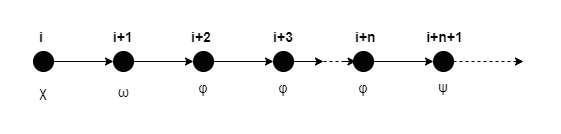
\includegraphics[width=0.8\textwidth]{Problem2-5.png}
\end{figure}